%
% File nacl2021.tex
%

% \documentclass[11pt,a4paper]{article}
\documentclass[11pt]{article}

% Remove the "review" option to generate the final version.
\usepackage[review]{template/naacl2021}

% \usepackage[hyperref]{template/eacl2021}

\usepackage{times}
\usepackage{latexsym}
% \renewcommand{\UrlFont}{\ttfamily\small}

% For proper rendering and hyphenation of words containing Latin characters (including in bib files)
\usepackage[T1]{fontenc}
% For Vietnamese characters
% \usepackage[T5]{fontenc}
% See https://www.latex-project.org/help/documentation/encguide.pdf for other character sets
\usepackage[UTF8]{ctex}

% This assumes your files are encoded as UTF8
\usepackage[utf8]{inputenc}

% This is not strictly necessary, and may be commented out,
% but it will improve the layout of the manuscript,
% and will typically save some space.
\usepackage{microtype}

% Graphics
\usepackage{graphicx}
\graphicspath{ {./figures/} }
%\newcommand\BibTeX{B\textsc{ib}\TeX}
\renewcommand{\tablename}{Table}
\renewcommand{\figurename}{Figure}

% If the title and author information does not fit in the area allocated, uncomment the following
%
%\setlength\titlebox{<dim>}
%
% and set <dim> to something 5cm or larger.
\title{Instructions for NAACL-HLT 2021 Proceedings}

% Author information can be set in various styles:
% For several authors from the same institution:
% \author{Author 1 \and ... \and Author n \\
%         Address line \\ ... \\ Address line}
% if the names do not fit well on one line use
%         Author 1 \\ {\bf Author 2} \\ ... \\ {\bf Author n} \\
% For authors from different institutions:
% \author{Author 1 \\ Address line \\  ... \\ Address line
%         \And  ... \And
%         Author n \\ Address line \\ ... \\ Address line}
% To start a seperate ``row'' of authors use \AND, as in
% \author{Author 1 \\ Address line \\  ... \\ Address line
%         \AND
%         Author 2 \\ Address line \\ ... \\ Address line \And
%         Author 3 \\ Address line \\ ... \\ Address line}

\author{First Author \\
	Affiliation / Address line 1 \\
	Affiliation / Address line 2 \\
	Affiliation / Address line 3 \\
	\texttt{email@domain} \\\And
	Second Author \\
	Affiliation / Address line 1 \\
	Affiliation / Address line 2 \\
	Affiliation / Address line 3 \\
	\texttt{email@domain} \\}

\date{}

\begin{document}
\maketitle


% Abstract
\begin{abstract}
	%auto-ignore
\label{sec:abstract}
This document is a supplement to the general instructions for *ACL authors. It contains instructions for using the \LaTeX{} style files for ACL conferences. 
The document itself conforms to its own specifications, and is therefore an example of what your manuscript should look like.
These instructions should be used both for papers submitted for review and for final versions of accepted papers.
\end{abstract}


% Main
%auto-ignore
\section{Introduction}
\label{sec:intro}



\subsection{Credits}

This document has been adapted
by Steven Bethard, Ryan Cotterrell and Rui Yan
from the instructions for earlier ACL and NAACL proceedings, including those for 
ACL 2019 by Douwe Kiela and Ivan Vuli\'{c},
NAACL 2019 by Stephanie Lukin and Alla Roskovskaya, 
ACL 2018 by Shay Cohen, Kevin Gimpel, and Wei Lu, 
NAACL 2018 by Margaret Michell and Stephanie Lukin,
2017/2018 (NA)ACL bibtex suggestions from Jason Eisner,
ACL 2017 by Dan Gildea and Min-Yen Kan, 
NAACL 2017 by Margaret Mitchell, 
ACL 2012 by Maggie Li and Michael White, 
ACL 2010 by Jing-Shing Chang and Philipp Koehn, 
ACL 2008 by Johanna D. Moore, Simone Teufel, James Allan, and Sadaoki Furui, 
ACL 2005 by Hwee Tou Ng and Kemal Oflazer, 
ACL 2002 by Eugene Charniak and Dekang Lin, 
and earlier ACL and EACL formats written by several people, including
John Chen, Henry S. Thompson and Donald Walker.
Additional elements were taken from the formatting instructions of the \emph{International Joint Conference on Artificial Intelligence} and the \emph{Conference on Computer Vision and Pattern Recognition}.

\subsection{Introduction}

The following instructions are directed to authors of papers submitted to EACL 2021 or accepted for publication in its proceedings.
All authors are required to adhere to these specifications.
Authors are required to provide a Portable Document Format (PDF) version of their papers.
\textbf{The proceedings are designed for printing on A4 paper.}

\subsection{Equations}

\begin{eqnarray}
	a  =  b + c \\
	=  y - z \\
	= \frac{p(x,y)}{p(y)}
\end{eqnarray}


\subsection{Electronically-available resources}

EACL provides this description and accompanying style files at
\begin{quote}
	\url{http://eacl2021.org/downloads/eacl2021-templates.zip}
\end{quote}
We strongly recommend the use of these style files, which have been appropriately tailored for the EACL 2021 proceedings.

\paragraph{\LaTeX-specific details:}
The templates include the \LaTeX2e{} source (\texttt{\small eacl2021.tex}),
the \LaTeX2e{} style file used to format it (\texttt{\small eacl2021.sty}),
an ACL bibliography style (\texttt{\small acl\_natbib.bst}),
an example bibliography (\texttt{\small acl2020.bib}),
and the bibliography for the ACL Anthology (\texttt{\small anthology.bib}).


%auto-ignore
\section{Related Work}
\label{sec:related}


\subsection{Preamble}

The first line of the file must be
\begin{quote}
	\begin{verbatim}
		\documentclass[11pt]{article}
	\end{verbatim}
\end{quote}

To load the style file in the review version:
\begin{quote}
	\begin{verbatim}
		\usepackage[review]{naacl2021}
	\end{verbatim}
\end{quote}
For the final version, omit the \verb|review| option:
\begin{quote}
	\begin{verbatim}
		\usepackage{naacl2021}
	\end{verbatim}
\end{quote}

To use Times Roman, put the following in the preamble:
\begin{quote}
	\begin{verbatim}
		\usepackage{times}
	\end{verbatim}
\end{quote}
(Alternatives like txfonts or newtx are also acceptable.)

Please see the \LaTeX{} source of this document for comments on other packages that may be useful.

Set the title and author using \verb|\title| and \verb|\author|. Within the author list, format multiple authors using \verb|\and| and \verb|\And| and \verb|\AND|; please see the \LaTeX{} source for examples.

By default, the box containing the title and author names is set to the minimum of 5 cm. If you need more space, include the following in the preamble:
\begin{quote}
	\begin{verbatim}
		\setlength\titlebox{<dim>}
	\end{verbatim}
\end{quote}
where \verb|<dim>| is replaced with a length. Do not set this length smaller than 5 cm.

%auto-ignore
\section{Methodology}
\label{sec:methodology}
 
 
 
\subsection{Formatting Instructions}
 
 Manuscripts must be in two-column format.
 Exceptions to the two-column format include the title, authors' names and complete addresses, which must be centered at the top of the first page, and any full-width figures or tables (see the guidelines in Section~\ref{ssec:title-authors}).
 \textbf{Type single-spaced.}
 Start all pages directly under the top margin.
 The manuscript should be printed single-sided and its length should not exceed the maximum page limit described in Section~\ref{sec:length}.
 Pages should be numbered in the version submitted for review, but \textbf{pages should not be numbered in the camera-ready version}.
 
 \paragraph{\LaTeX-specific details:}
 The style files will generate page numbers when {\small\verb|\aclfinalcopy|} is commented out, and remove them otherwise.
 
 
 \subsection{File Format}
 \label{sect:pdf}
 
 For the production of the electronic manuscript you must use Adobe's Portable Document Format (PDF).
 Please make sure that your PDF file includes all the necessary fonts (especially tree diagrams, symbols, and fonts with Asian characters).
 When you print or create the PDF file, there is usually an option in your printer setup to include none, all or just non-standard fonts.
 Please make sure that you select the option of including ALL the fonts.
 \textbf{Before sending it, test your PDF by printing it from a computer different from the one where it was created.}
 Moreover, some word processors may generate very large PDF files, where each page is rendered as an image.
 Such images may reproduce poorly.
 In this case, try alternative ways to obtain the PDF.
 One way on some systems is to install a driver for a postscript printer, send your document to the printer specifying ``Output to a file'', then convert the file to PDF.
 
 It is of utmost importance to specify the \textbf{A4 format} (21 cm x 29.7 cm) when formatting the paper.
 Print-outs of the PDF file on A4 paper should be identical to the hardcopy version.
 If you cannot meet the above requirements about the production of your electronic submission, please contact the publication chairs as soon as possible.
 
 \paragraph{\LaTeX-specific details:}
 PDF files are usually produced from \LaTeX{} using the \texttt{\small pdflatex} command.
 If your version of \LaTeX{} produces Postscript files, \texttt{\small ps2pdf} or \texttt{\small dvipdf} can convert these to PDF.
 To ensure A4 format in \LaTeX, use the command {\small\verb|\special{papersize=210mm,297mm}|}
 in the \LaTeX{} preamble (below the {\small\verb|\usepackage|} commands) and use \texttt{\small dvipdf} and/or \texttt{\small pdflatex}; or specify \texttt{\small -t a4} when working with \texttt{\small dvips}.
 
 \subsection{Layout}
 \label{ssec:layout}
 
 Format manuscripts two columns to a page, in the manner these
 instructions are formatted.
 The exact dimensions for a page on A4 paper are:
 
 \begin{itemize}
 	\item Left and right margins: 2.5 cm
 	\item Top margin: 2.5 cm
 	\item Bottom margin: 2.5 cm
 	\item Column width: 7.7 cm
 	\item Column height: 24.7 cm
 	\item Gap between columns: 0.6 cm
 \end{itemize}
 
 \noindent Papers should not be submitted on any other paper size.
 If you cannot meet the above requirements about the production of your electronic submission, please contact the publication chairs above as soon as possible.
 
 \subsection{Fonts}
 
 For reasons of uniformity, Adobe's \textbf{Times Roman} font should be used.
 If Times Roman is unavailable, you may use Times New Roman or \textbf{Computer Modern Roman}.
 
 Table~\ref{font-table} specifies what font sizes and styles must be used for each type of text in the manuscript.
 
 \begin{table}
 	\centering
 	\begin{tabular}{lrl}
 		\hline \textbf{Type of Text} & \textbf{Font Size} & \textbf{Style} \\ \hline
 		paper title & 15 pt & bold \\
 		author names & 12 pt & bold \\
 		author affiliation & 12 pt & \\
 		the word ``Abstract'' & 12 pt & bold \\
 		section titles & 12 pt & bold \\
 		subsection titles & 11 pt & bold \\
 		document text & 11 pt  &\\
 		captions & 10 pt & \\
 		abstract text & 10 pt & \\
 		bibliography & 10 pt & \\
 		footnotes & 9 pt & \\
 		\hline
 	\end{tabular}
 	\caption{\label{font-table} Font guide. }
 \end{table}
 
 \paragraph{\LaTeX-specific details:}
 To use Times Roman in \LaTeX2e{}, put the following in the preamble:
 \begin{quote}
 	\small
 	\begin{verbatim}
 		\usepackage{times}
 		\usepackage{latexsym}
 	\end{verbatim}
 \end{quote}
 
 
 \subsection{Ruler}
 A printed ruler (line numbers in the left and right margins of the article) should be presented in the version submitted for review, so that reviewers may comment on particular lines in the paper without circumlocution.
 The presence or absence of the ruler should not change the appearance of any other content on the page.
 The camera ready copy should not contain a ruler.
 
 \paragraph{Reviewers:}
 note that the ruler measurements may not align well with lines in the paper -- this turns out to be very difficult to do well when the paper contains many figures and equations, and, when done, looks ugly.
 In most cases one would expect that the approximate location will be adequate, although you can also use fractional references (\emph{e.g.}, this line ends at mark $295.5$).
 
 \paragraph{\LaTeX-specific details:}
 The style files will generate the ruler when {\small\verb|\aclfinalcopy|} is commented out, and remove it otherwise.
 
 \subsection{Title and Authors}
 \label{ssec:title-authors}
 
 Center the title, author's name(s) and affiliation(s) across both columns.
 Do not use footnotes for affiliations.
 Place the title centered at the top of the first page, in a 15-point bold font.
 Long titles should be typed on two lines without a blank line intervening.
 Put the title 2.5 cm from the top of the page, followed by a blank line, then the author's names(s), and the affiliation on the following line.
 Do not use only initials for given names (middle initials are allowed).
 Do not format surnames in all capitals (\emph{e.g.}, use ``Mitchell'' not ``MITCHELL'').
 Do not format title and section headings in all capitals except for proper names (such as ``BLEU'') that are
 conventionally in all capitals.
 The affiliation should contain the author's complete address, and if possible, an electronic mail address.
 
 The title, author names and addresses should be completely identical to those entered to the electronical paper submission website in order to maintain the consistency of author information among all publications of the conference.
 If they are different, the publication chairs may resolve the difference without consulting with you; so it is in your own interest to double-check that the information is consistent.
 
 Start the body of the first page 7.5 cm from the top of the page.
 \textbf{Even in the anonymous version of the paper, you should maintain space for names and addresses so that they will fit in the final (accepted) version.}
 
 
 \subsection{Abstract}
 Use two-column format when you begin the abstract.
 Type the abstract at the beginning of the first column.
 The width of the abstract text should be smaller than the
 width of the columns for the text in the body of the paper by 0.6 cm on each side.
 Center the word \textbf{Abstract} in a 12 point bold font above the body of the abstract.
 The abstract should be a concise summary of the general thesis and conclusions of the paper.
 It should be no longer than 200 words.
 The abstract text should be in 10 point font.
 
 \subsection{Text}
 Begin typing the main body of the text immediately after the abstract, observing the two-column format as shown in the present document.
 
 Indent 0.4 cm when starting a new paragraph.
 
 \subsection{Sections}
 
 Format section and subsection headings in the style shown on the present document.
 Use numbered sections (Arabic numerals) to facilitate cross references.
 Number subsections with the section number and the subsection number separated by a dot, in Arabic numerals.
 
 \subsection{Footnotes}
 Put footnotes at the bottom of the page and use 9 point font.
 They may be numbered or referred to by asterisks or other symbols.\footnote{This is how a footnote should appear.}
 Footnotes should be separated from the text by a line.\footnote{Note the line separating the footnotes from the text.}
 
 \subsection{Graphics}
 
 
 \begin{figure}[h!]
 	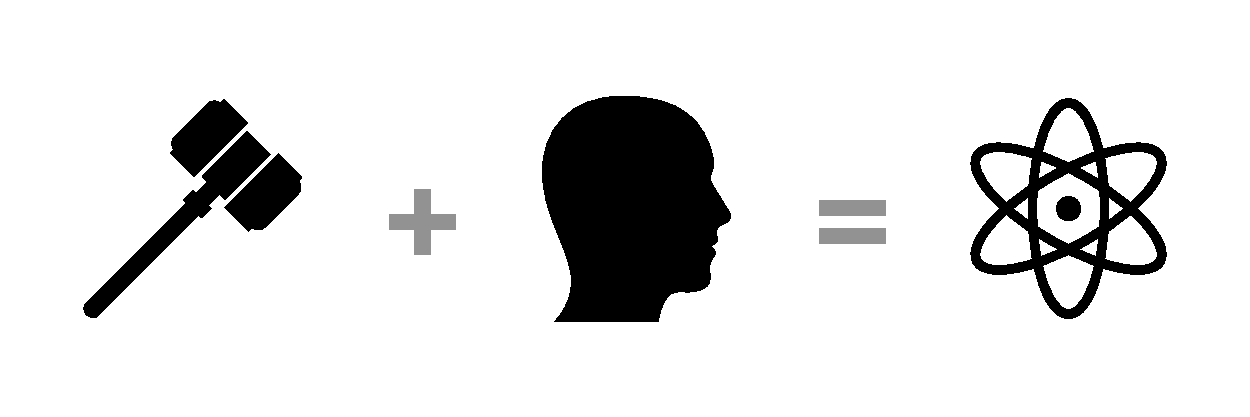
\includegraphics[width=0.5\textwidth]{wisdom.pdf}
 	\caption{Physically increasing wisdom.}
 	\label{fig:wisdom}
 \end{figure}

 Place figures, tables, and photographs in the paper near where they are first discussed, rather than at the end, if possible.
 Wide illustrations may run across both columns.
 Color is allowed, but adhere to Section~\ref{ssec:accessibility}'s guidelines on accessibility.
 
 
 
 \paragraph{Captions:}
 Provide a caption for every illustration; number each one sequentially in the form:
 ``Figure 1. Caption of the Figure.''
 ``Table 1. Caption of the Table.''
 Type the captions of the figures and tables below the body, using 10 point text.
 Captions should be placed below illustrations.
 Captions that are one line are centered (see Table~\ref{font-table}).
 Captions longer than one line are left-aligned (see Table~\ref{tab:accents}).
 
 \begin{table}
 	\centering
 	\begin{tabular}{lc}
 		\hline
 		\textbf{Command} & \textbf{Output}\\
 		\hline
 		\verb|{\"a}| & {\"a} \\
 		\verb|{\^e}| & {\^e} \\
 		\verb|{\`i}| & {\`i} \\ 
 		\verb|{\.I}| & {\.I} \\ 
 		\verb|{\o}| & {\o} \\
 		\verb|{\'u}| & {\'u}  \\ 
 		\verb|{\aa}| & {\aa}  \\\hline
 	\end{tabular}
 	\begin{tabular}{lc}
 		\hline
 		\textbf{Command} & \textbf{Output}\\
 		\hline
 		\verb|{\c c}| & {\c c} \\ 
 		\verb|{\u g}| & {\u g} \\ 
 		\verb|{\l}| & {\l} \\ 
 		\verb|{\~n}| & {\~n} \\ 
 		\verb|{\H o}| & {\H o} \\ 
 		\verb|{\v r}| & {\v r} \\ 
 		\verb|{\ss}| & {\ss} \\
 		\hline
 	\end{tabular}
 	\caption{Example commands for accented characters, to be used in, \emph{e.g.}, \BibTeX\ names.}\label{tab:accents}
 \end{table}
 
 \paragraph{\LaTeX-specific details:}
 The style files are compatible with the caption and subcaption packages; do not add optional arguments.
 \textbf{Do not override the default caption sizes.}
 
 
 \subsection{Hyperlinks}
 Within-document and external hyperlinks are indicated with Dark Blue text, Color Hex \#000099.
 
 \subsection{Citations}
 Citations within the text appear in parentheses as~\citep{Gusfield:97} or, if the author's name appears in the text itself, as \citet{Gusfield:97}.
 Append lowercase letters to the year in cases of ambiguities.  
 Treat double authors as in~\citep{Aho:72}, but write as in~\citep{Chandra:81} when more than two authors are involved. Collapse multiple citations as in~\citep{Gusfield:97,Aho:72}. 
 
 Refrain from using full citations as sentence constituents.
 Instead of
 \begin{quote}
 	``\citep{Gusfield:97} showed that ...''
 \end{quote}
 write
 \begin{quote}
 	``\citet{Gusfield:97} showed that ...''
 \end{quote}
 
 \begin{table*}
 	\centering
 	\begin{tabular}{lll}
 		\hline
 		\textbf{Output} & \textbf{natbib command} & \textbf{Old ACL-style command}\\
 		\hline
 		\citep{Gusfield:97} & \small\verb|\citep| & \small\verb|\cite| \\
 		\citealp{Gusfield:97} & \small\verb|\citealp| & no equivalent \\
 		\citet{Gusfield:97} & \small\verb|\citet| & \small\verb|\newcite| \\
 		\citeyearpar{Gusfield:97} & \small\verb|\citeyearpar| & \small\verb|\shortcite| \\
 		\hline
 	\end{tabular}
 	\caption{\label{citation-guide}
 		Citation commands supported by the style file.
 		The style is based on the natbib package and supports all natbib citation commands.
 		It also supports commands defined in previous ACL style files for compatibility.
 	}
 \end{table*}
 
 \paragraph{\LaTeX-specific details:}
 Table~\ref{citation-guide} shows the syntax supported by the style files.
 We encourage you to use the natbib styles.
 You can use the command {\small\verb|\citet|} (cite in text) to get ``author (year)'' citations as in \citet{Gusfield:97}.
 You can use the command {\small\verb|\citep|} (cite in parentheses) to get ``(author, year)'' citations as in \citep{Gusfield:97}.
 You can use the command {\small\verb|\citealp|} (alternative cite without  parentheses) to get ``author year'' citations (which is useful for  using citations within parentheses, as in \citealp{Gusfield:97}).
 
 
 \subsection{References}
 Gather the full set of references together under the heading \textbf{References}; place the section before any Appendices. 
 Arrange the references alphabetically by first author, rather than by order of occurrence in the text.
 
 Provide as complete a citation as possible, using a consistent format, such as the one for \emph{Computational Linguistics\/} or the one in the  \emph{Publication Manual of the American 
 	Psychological Association\/}~\citep{APA:83}.
 Use full names for authors, not just initials.
 
 Submissions should accurately reference prior and related work, including code and data.
 If a piece of prior work appeared in multiple venues, the version that appeared in a refereed, archival venue should be referenced.
 If multiple versions of a piece of prior work exist, the one used by the authors should be referenced.
 Authors should not rely on automated citation indices to provide accurate references for prior and related work.
 
 The following text cites various types of articles so that the references section of the present document will include them.
 \begin{itemize}
 	\item Example article in journal: \citep{Ando2005}.
 	\item Example article in proceedings, with location: \citep{borschinger-johnson-2011-particle}.
 	\item Example article in proceedings, without location: \citep{andrew2007scalable}.
 	\item Example arxiv paper: \citep{rasooli-tetrault-2015}. 
 \end{itemize}
 
 
 \paragraph{\LaTeX-specific details:}
 The \LaTeX{} and Bib\TeX{} style files provided roughly follow the American Psychological Association format.
 If your own bib file is named \texttt{\small eacl2021.bib}, then placing the following before any appendices in your \LaTeX{}  file will generate the references section for you:
 \begin{quote}\small
 	\verb|\bibliographystyle{acl_natbib}|\\
 	\verb|\bibliography{eacl2021}|
 \end{quote}
 
 You can obtain the complete ACL Anthology as a Bib\TeX\ file from \url{https://aclweb.org/anthology/anthology.bib.gz}.
 To include both the anthology and your own bib file, use the following instead of the above.
 \begin{quote}\small
 	\verb|\bibliographystyle{acl_natbib}|\\
 	\verb|\bibliography{anthology,eacl2021}|
 \end{quote}
 
 
 \subsection{Digital Object Identifiers}
 As part of our work to make ACL materials more widely used and cited outside of our discipline, ACL has registered as a CrossRef member, as a registrant of Digital Object Identifiers (DOIs), the standard for registering permanent URNs for referencing scholarly materials.
 
 All camera-ready references are required to contain the appropriate DOIs (or as a second resort, the hyperlinked ACL Anthology Identifier) to all cited works.
 Appropriate records should be found for most materials in the current ACL Anthology at \url{http://aclanthology.info/}.
 As examples, we cite \citep{goodman-etal-2016-noise} to show you how papers with a DOI will appear in the bibliography.
 We cite \citep{harper-2014-learning} to show how papers without a DOI but with an ACL Anthology Identifier will appear in the bibliography.
 
 \paragraph{\LaTeX-specific details:}
 Please ensure that you use Bib\TeX\ records that contain DOI or URLs for any of the ACL materials that you reference.
 If the Bib\TeX{} file contains DOI fields, the paper title in the references section will appear as a hyperlink to the DOI, using the hyperref \LaTeX{} package.
 
 
 \subsection{Appendices}
 Appendices, if any, directly follow the text and the
 references (but only in the camera-ready; see Appendix~\ref{sec:appendix}).
 Letter them in sequence and provide an informative title:
 \textbf{Appendix A. Title of Appendix}.
 
%auto-ignore
\section{Experiments}
\label{sec:experiment}


\subsection{Hyperlinks}

Users of older versions of \LaTeX{} may encounter the following error during compilation: 
\begin{quote}
	\tt\verb|\pdfendlink| ended up in different nesting level than \verb|\pdfstartlink|.
\end{quote}
This happens when pdf\LaTeX{} is used and a citation splits across a page boundary. The best way to fix this is to upgrade \LaTeX{} to 2018-12-01 or later.

\subsection{Citations}

\begin{table*}
	\centering
	\begin{tabular}{lll}
		\hline
		\textbf{Output} & \textbf{natbib command} & \textbf{Old ACL-style command}\\
		\hline
		\citep{Gusfield:97} & \verb|\citep| & \verb|\cite| \\
		\citealp{Gusfield:97} & \verb|\citealp| & no equivalent \\
		\citet{Gusfield:97} & \verb|\citet| & \verb|\newcite| \\
		\citeyearpar{Gusfield:97} & \verb|\citeyearpar| & \verb|\shortcite| \\
		\hline
	\end{tabular}
	\caption{\label{citation-guide}
		Citation commands supported by the style file.
		The style is based on the natbib package and supports all natbib citation commands.
		It also supports commands defined in previous ACL style files for compatibility.
	}
\end{table*}

Table~\ref{citation-guide} shows the syntax supported by the style files.
We encourage you to use the natbib styles.
You can use the command \verb|\citet| (cite in text) to get ``author (year)'' citations, like this citation to a paper by \citet{Gusfield:97}.
You can use the command \verb|\citep| (cite in parentheses) to get ``(author, year)'' citations \citep{Gusfield:97}.
You can use the command \verb|\citealp| (alternative cite without parentheses) to get ``author, year'' citations, which is useful for using citations within parentheses (e.g. \citealp{Gusfield:97}).

\subsection{References}

\nocite{Ando2005,borschinger-johnson-2011-particle,andrew2007scalable,rasooli-tetrault-2015,goodman-etal-2016-noise,harper-2014-learning}

The \LaTeX{} and Bib\TeX{} style files provided roughly follow the American Psychological Association format.
If your own bib file is named \texttt{custom.bib}, then placing the following before any appendices in your \LaTeX{} file will generate the references section for you:
\begin{quote}
	\begin{verbatim}
		\bibliographystyle{acl_natbib}
		\bibliography{custom}
	\end{verbatim}
\end{quote}

You can obtain the complete ACL Anthology as a Bib\TeX{} file from \url{https://aclweb.org/anthology/anthology.bib.gz}.
To include both the Anthology and your own .bib file, use the following instead of the above.
\begin{quote}
	\begin{verbatim}
		\bibliographystyle{acl_natbib}
		\bibliography{anthology,custom}
	\end{verbatim}
\end{quote}

Please see Section~\ref{sec:bibtex} for information on preparing Bib\TeX{} files.


%auto-ignore
\section{Conclusion}
\label{sec:conclusion}

\paragraph{Bib\TeX{} Files}
\label{sec:bibtex}

Unicode cannot be used in Bib\TeX{} entries, and some ways of typing special characters can disrupt Bib\TeX's alphabetization. The recommended way of typing special characters is shown in Table~\ref{tab:accents}.

Please ensure that Bib\TeX{} records contain DOIs or URLs when possible, and for all the ACL materials that you reference.
Use the \verb|doi| field for DOIs and the \verb|url| field for URLs.
If a Bib\TeX{} entry has a URL or DOI field, the paper title in the references section will appear as a hyperlink to the paper, using the hyperref \LaTeX{} package.

\section*{Acknowledgements}

This document has been adapted
by Steven Bethard, Ryan Cotterell and Rui Yan
from the instructions for earlier ACL and NAACL proceedings, including those for 
ACL 2019 by Douwe Kiela and Ivan Vuli\'{c},
NAACL 2019 by Stephanie Lukin and Alla Roskovskaya, 
ACL 2018 by Shay Cohen, Kevin Gimpel, and Wei Lu, 
NAACL 2018 by Margaret Mitchell and Stephanie Lukin,
Bib\TeX{} suggestions for (NA)ACL 2017/2018 from Jason Eisner,
ACL 2017 by Dan Gildea and Min-Yen Kan, 
NAACL 2017 by Margaret Mitchell, 
ACL 2012 by Maggie Li and Michael White, 
ACL 2010 by Jing-Shin Chang and Philipp Koehn, 
ACL 2008 by Johanna D. Moore, Simone Teufel, James Allan, and Sadaoki Furui, 
ACL 2005 by Hwee Tou Ng and Kemal Oflazer, 
ACL 2002 by Eugene Charniak and Dekang Lin, 
and earlier ACL and EACL formats written by several people, including
John Chen, Henry S. Thompson and Donald Walker.
Additional elements were taken from the formatting instructions of the \emph{International Joint Conference on Artificial Intelligence} and the \emph{Conference on Computer Vision and Pattern Recognition}.



\bibliography{bibliography/anthology,bibliography/custom}
\bibliographystyle{template/acl_natbib}

\appendix


% Appendix
\appendix
%auto-ignore
\section{Appendices}
\label{sec:appendix}

Use \verb|\appendix| before any appendix section to switch the section numbering over to letters. See Appendix~\ref{sec:appendix} for an example.

%auto-ignore
\section{Supplemental Material}
\label{sec:supplemental}



\paragraph{Notable changes} in the templates \url{https://2021.naacl.org/calls/style-and-formatting/} (by Matt Post and David Chiang) are:

NAACL-HLT 2021 is using latex templates based on the new organization of templates and formatting guidelines for *ACL papers here\url{https://github.com/acl-org/ACLPUB}.

We now use the “lineno” package instead of writing pseudo-numbers down the margins. Line numbers now line up, and many other simplifications were enabled by this change.

We will not use the \verb|\aclfinalcopy| command. Instead, the review copy (anonymized, page and line numbers) is enabled by passing “review” as an “acl” package argument:

\begin{verbatim}
    \usepackage[review]{acl}
\end{verbatim}

There is no \verb|\aclpaperid| macro. Softconf will add the submission ID stamp.

A few bug fixes that have cropped up over the years and then sometimes inadvertently reintroduced.



\end{document}
